\section{Introducción}

\begin{frame}
	\frametitle{Escasez de agua}
	Para enfrentar la creciente escasez de agua se han desarrollado diversas tecnologías de desalinización (cualquier proceso que elimine las sales del agua)\\[5mm]
	\begin{columns}
		\begin{column}{0.5\linewidth}
			\centering
			\begin{figure}
				\centering
				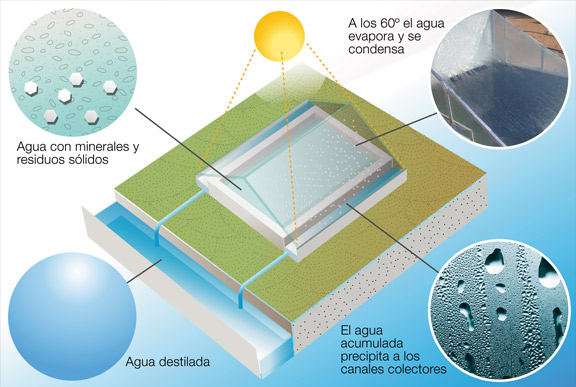
\includegraphics[
					height=50mm,
					width=\linewidth,
					keepaspectratio
				]{destilador-solar.jpg}
				\caption{Destilador solar pasivo}
			\end{figure}
		\end{column}
		\begin{column}{0.5\linewidth}
			\centering
			\begin{figure}
				\centering
				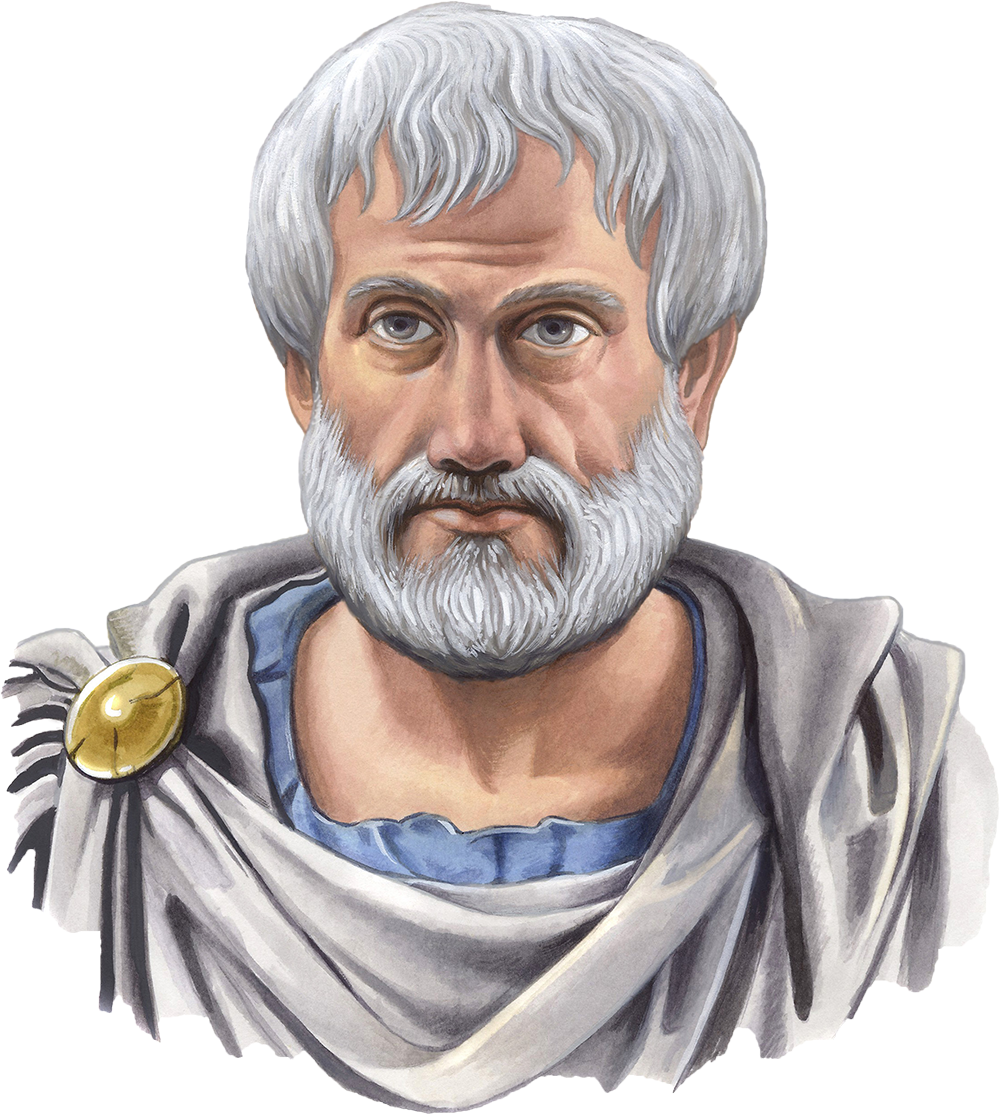
\includegraphics[
					height=50mm,
					width=\linewidth,
					keepaspectratio
				]{aristoteles.png}
				\caption{Aristóteles}
			\end{figure}
		\end{column}
	\end{columns}
\end{frame}

\begin{frame}
    \frametitle{Destilador solar pasivo}
    \begin{columns}
        \begin{column}{0.5\textwidth}
            \textbf{\large Ventajas}
            
            \begin{itemize}
                \item Alimentado por una fuente renovable de energía
                \item Emisiones nulas de \acrfull{gei}
                \item Eliminación de agentes patógenos
                \item Costos de mantenimiento bajos
            \end{itemize}
            \vspace*{3mm}
            \textbf{\large Desventajas}
            
            \begin{itemize}
                \item Producción más cara a otras tecnologías
                \item Baja productividad contra otras tecnologías
            \end{itemize}
        \end{column}
        
        \begin{column}{0.5\textwidth}
            \centering
            \begin{figure}
                \centering
                
\includegraphics[
                    width=0.9\linewidth,
                    keepaspectratio
                ]{cero-emisiones-netas.png}
                \caption{Emisiones netas cero para 2050}
            \end{figure}
        \end{column}
    \end{columns}
\end{frame}

\begin{frame}
	\frametitle{Destilador solar activo}
	
	Cuando a un destilador solar se le incorpora cualquier elemento que proporcione mayor energía aumentando así su productividad, se denominará como \textbf{destilador solar activo}.
	\vspace*{2mm}
	\begin{columns}
		\begin{column}{0.5\textwidth}
			\centering
			\begin{figure}
				\centering
				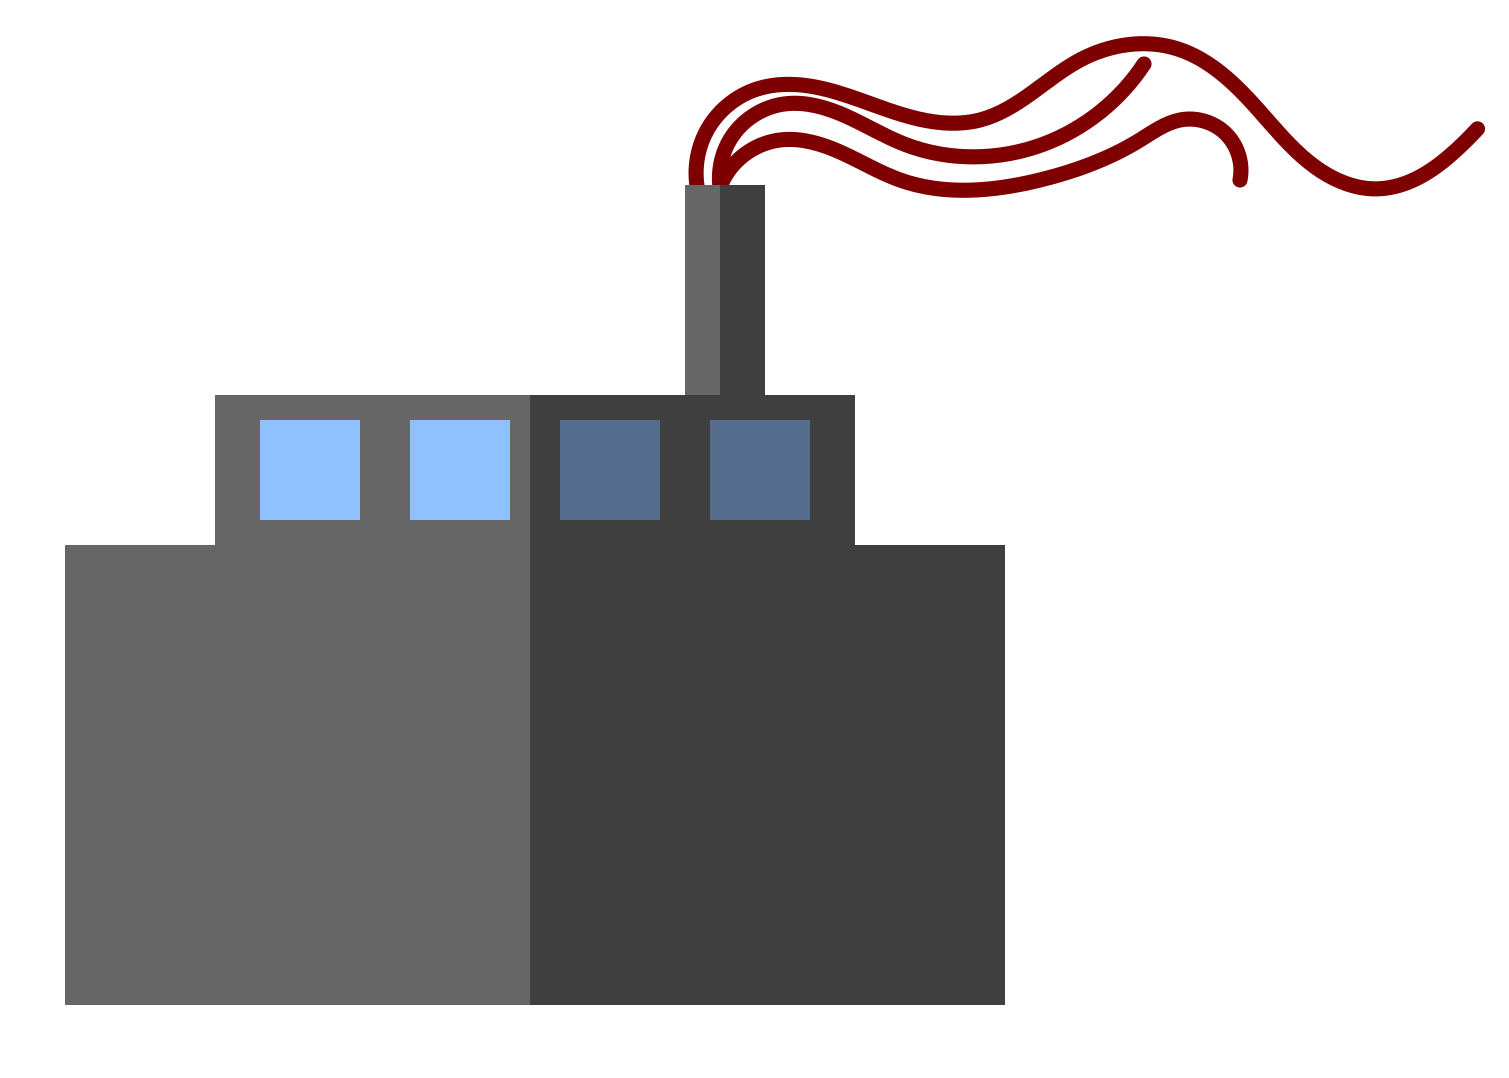
\includegraphics[
					height=50mm,
					width=\linewidth,
					keepaspectratio
				]{industria.png}
				\caption{Calor residual}
			\end{figure}
		\end{column}			
		\begin{column}{0.5\textwidth}
			\centering
			\begin{figure}
				\centering
				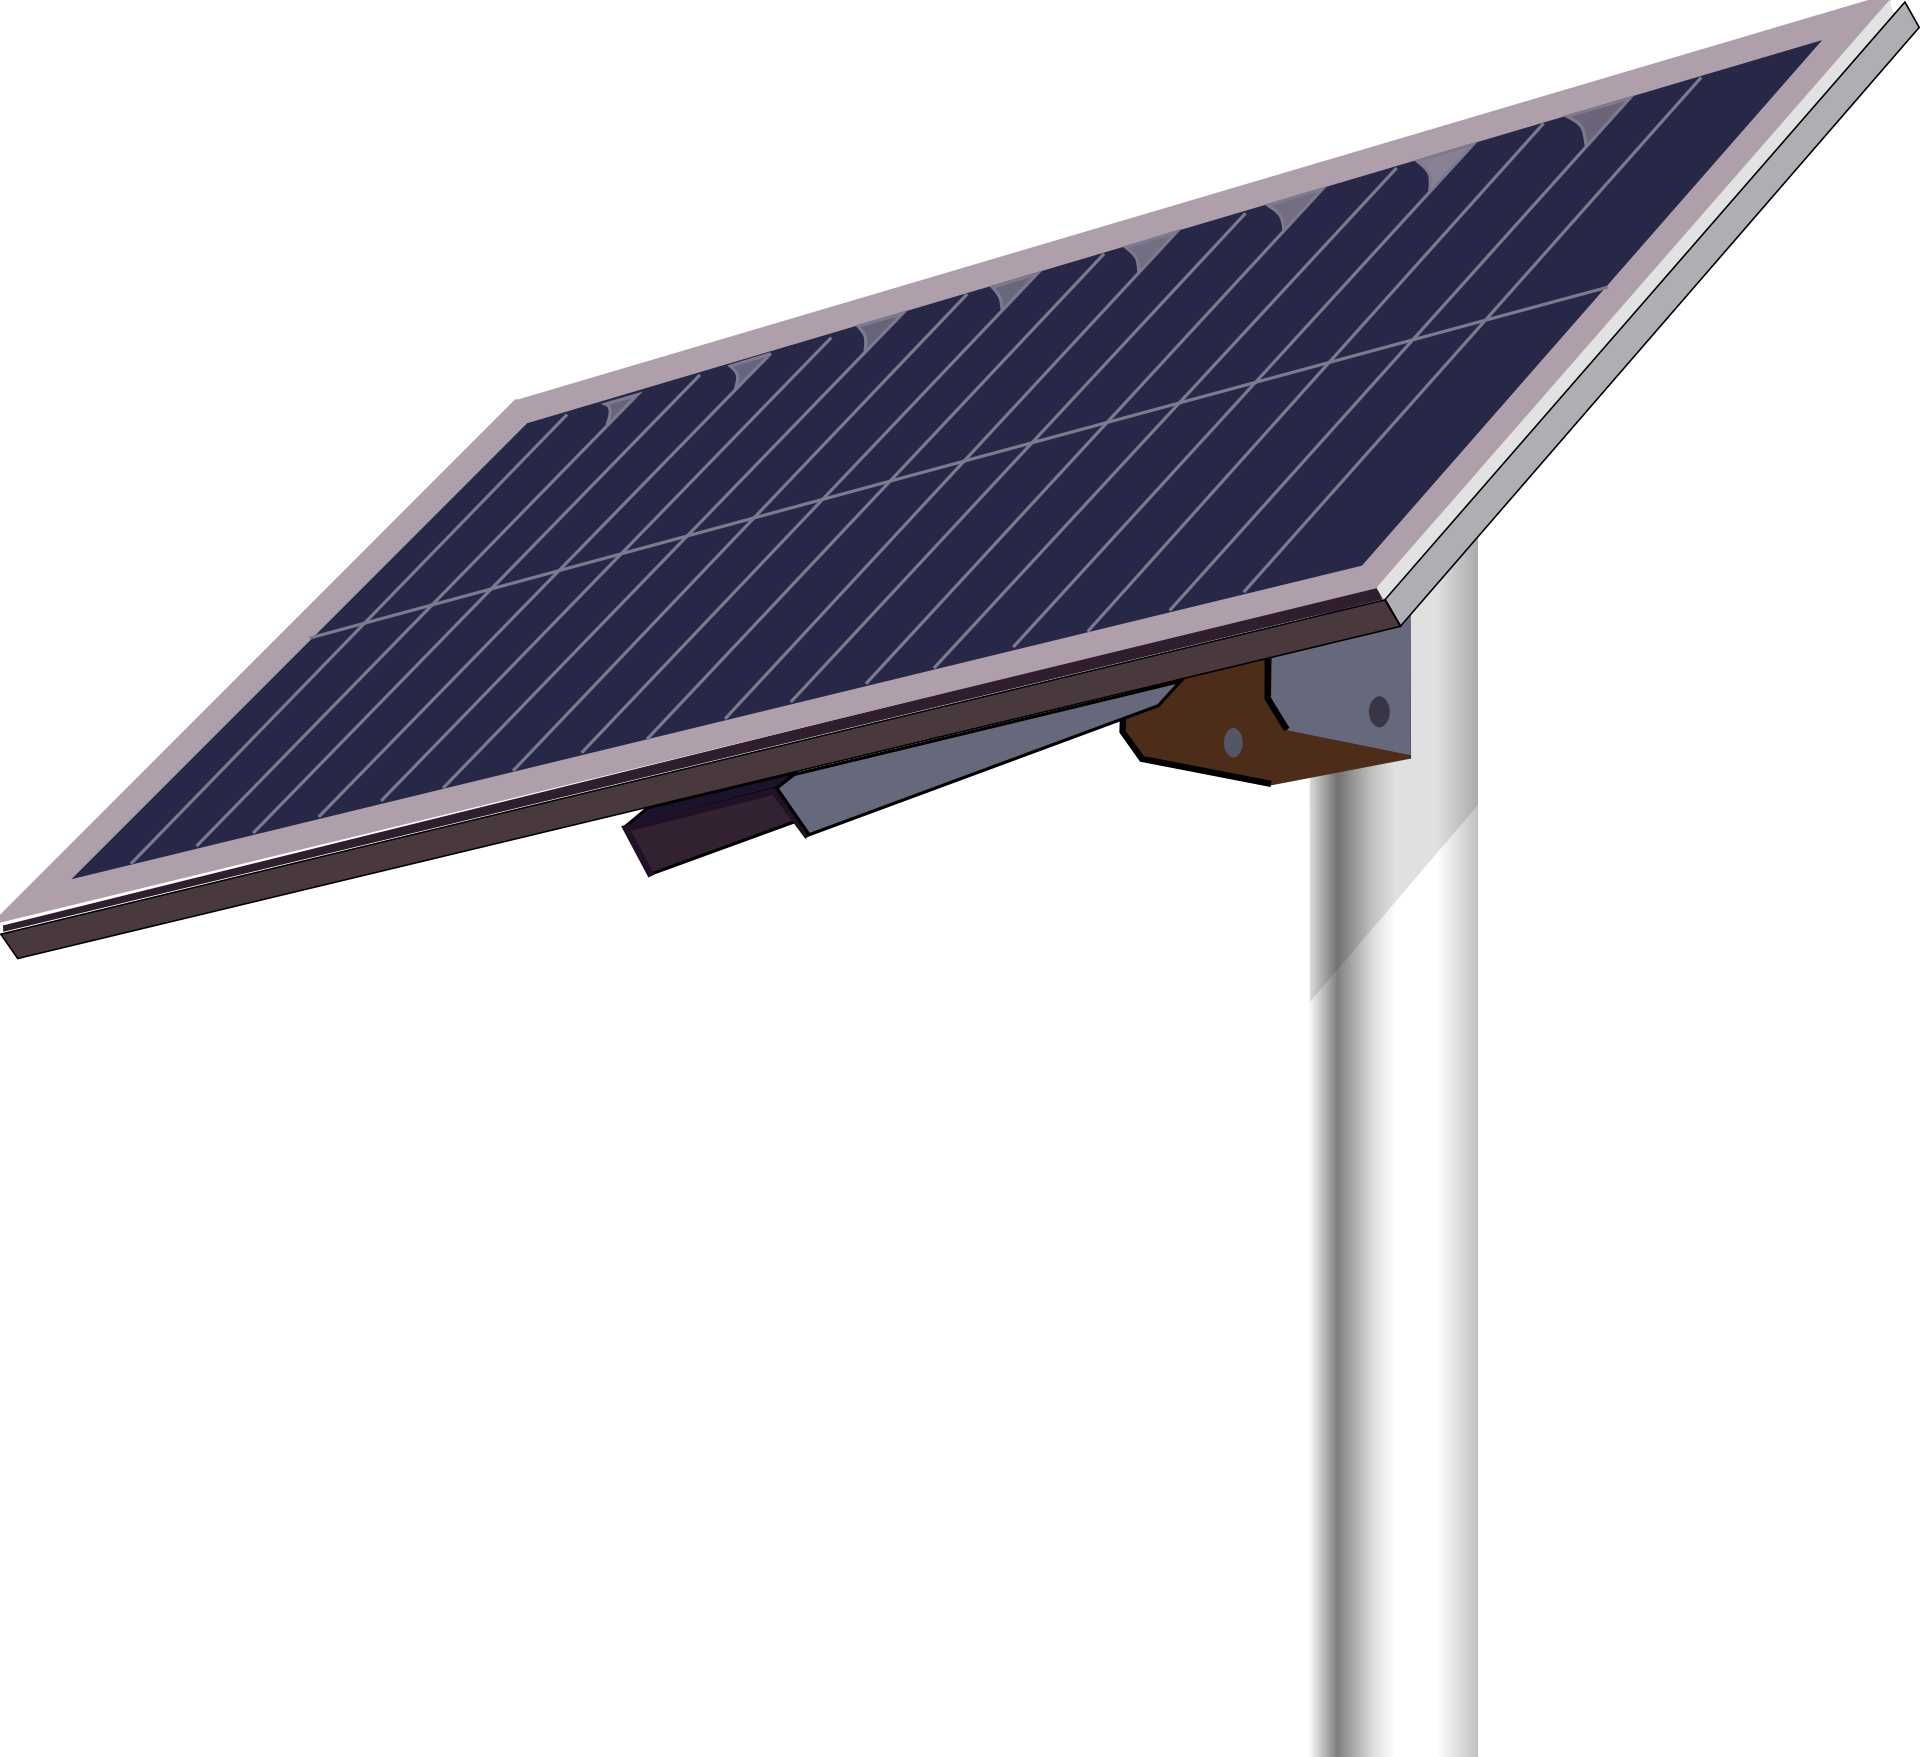
\includegraphics[
					height=50mm,
					width=\linewidth,
					keepaspectratio
				]{panel-solar.png}
				\caption{Fuente de energía secundaria}
			\end{figure}
		\end{column}
	\end{columns}
\end{frame}